\documentclass[a4paper]{article}
\usepackage[italian]{babel}
\usepackage[T1]{fontenc}
\usepackage[utf8]{inputenc}
\usepackage{graphicx}
\usepackage[margin=1in]{geometry}
\usepackage{makecell}
%\usepackage[svgnames,table]{xcolor}
\usepackage[table]{xcolor}
% --- Per lo sfondo
%\usepackage{eso-pic,graphicx}
% ---
\usepackage{setspace}

\usepackage{tabularx} 

\usepackage[hidelinks]{hyperref}
\usepackage{array}

\usepackage{fancyhdr}
\usepackage{float}

% Definizione comandi personali - Team
\newcommand{\FP}{Francesco Protopapa}
\newcommand{\GC}{Greta Cavedon}
\newcommand{\LW}{Luciano Wu}
\newcommand{\PV}{Pietro Villatora}
\newcommand{\EP}{Edoardo Pavan}
\newcommand{\MG}{Michele Gatto}
\newcommand{\MB}{Matteo Basso}

% Definizione File
\newcommand{\G}{\textit{Glossario v1.0.0}}
\newcommand{\AdR}{\textit{Analisi dei Requisiti v1.0.0}}
\newcommand{\PdP}{\textit{Piano di Progetto v1.0.0}}
\newcommand{\PdQ}{\textit{Piano di Qualifica v1.0.0}}
\newcommand{\SdF}{\textit{Studio di fattibilità v1.0.0}}
\newcommand{\NdP}{\textit{Norme di Progetto v1.0.0}}

% Definizione ruoli
\newcommand{\AN}{Analista}
\newcommand{\VE}{Verificatore}
\newcommand{\AM}{Amministratore}
\newcommand{\RE}{Responsabile}
\newcommand{\PT}{Progettista}
\newcommand{\PR}{Programmatore}

\newcommand{\glo}{\textsuperscript{G}}

%Abbreviaizoni requisiti
\newcommand{\Ob}{Obbligatorio}
\newcommand{\De}{Desiderabile}
\newcommand{\Fa}{Facoltativo}

%Abbrevizioni fonti requisiti
\newcommand{\Di}{Decisione interna}
\newcommand{\Vi}{Verbale interno}
\newcommand{\Ve}{Verbale esterno}
\newcommand{\Ca}{Capitolato}

%link in blu
\newcommand{\mylink}[1]{\color{blue}\url{#1}\color{black}}
\makeindex

\usepackage{longtable}

% Per evidenziare il testo
\usepackage{tcolorbox}



\setcounter{secnumdepth}{4}
\setcounter{tocdepth}{4}

\begin{document}

	% Intro documento 

\begin{center}

\begin{figure}
\centering

\includegraphics[scale=0.05]{Contenuto/Immagini/DreamTeam.png} 
\end{figure}

{\Huge{\textbf{Norme di Progetto}}} \\ [1cm]

\begin{table}[htbp]
\centering
\begin{tabular}{r|c}
\multicolumn{2}{c}{\textbf{Informazioni sul Documento}} \\
\hline \\
\textbf{Versione} & 3.0.0 \\ \rule{0pt}{3ex}    
\textbf{Data di approvazione} & 2022-06-18  \\ \rule{0pt}{2ex} 
\textbf{Approvatori} & \MB{} \\ \rule{0pt}{3ex}      
\textbf{Redattori} & \MG{} \\ \rule{0pt}{2ex}   
& \PV{} \\ \rule{0pt}{3ex}    
\textbf{Verificatori} 
  & \GC{} \\ \rule{0pt}{2ex}
& \EP{} \\ \rule{0pt}{2ex} 
      
\textbf{Uso} & Interno \\ \rule{0pt}{3ex}    
\textbf{Distribuzione} & Prof. Vardanega Tullio \\ \rule{0pt}{2ex}   
& Prof. Cardin Riccardo \\ \rule{0pt}{2ex}   
& Gruppo \textit{DreamTeam} \\ \rule{0pt}{0.1cm}   
\end{tabular} \\ [0.5cm]
\end{table}

\textsl{ e-mail: \href{mailto:dreamteam.unipd@gmail.com}{dreamteam.unipd@gmail.com} } \\[2cm]
\end{center}
\pagebreak	
	% Inserimento di header e footer

\pagestyle{fancy}
\fancyhf{}
\rhead{Piano di Progetto}
\lhead{
\includegraphics[scale=0.015]{Sezioni/images/DreamTeam.png}}
\rfoot{\thepage}
\setlength{\headheight}{35pt}


%\cfoot{Pagina \thepage}
%\setlength{\headheight}{35pt}
%\setcounter{tocdepth}{5}
%\setcounter{secnumdepth}{5}
%\renewcommand{\footrulewidth}{0.4pt}
	% Registro Modifiche

\definecolor{darkblue}{cmyk}{99, 99, 0, 71}

{\LARGE{\textbf{Registro delle Modifiche}}} \\
\begin{table}[!htbp]
\rowcolors{2}{gray!25}{white}
\renewcommand{\arraystretch}{1.5}
\begin{tabular}{ m{0.1\textwidth}<{\centering}  m{0.11\textwidth}<{\centering}  m{0.2\textwidth}<{\centering}  m{0.17\textwidth}<{\centering}  m{0.3\textwidth}<{\centering} }
	\rowcolor{darkblue}
	\textcolor{white}{\textbf{Versione}} &\textcolor{white}{\textbf{Data}}& \textcolor{white}{\textbf{Nominativo}} & \textcolor{white}{\textbf{Ruolo}}&\textcolor{white}{\textbf{Descrizione}}\\ 
	v1.0.0& 2022-01- & \shortstack{ \\ XX} &\shortstack{ \\ \RE{} } & Approvazione del documento \\

	v0.0.1& 2022-01-14 & \shortstack{ \\ \GC{}} &\shortstack{ \\ \AN{} } & Realizzazione struttura in Latex e stesura documento; \VE: \textit{}\\

\end{tabular}
\end{table}

\pagebreak	
		
	% indice
	\renewcommand{\contentsname}{Indice}
	\tableofcontents	
	\pagebreak
	
	% contenuto del documento, ogni sezione in un file
	\section{Introduzione}

\subsection{Scopo del Documento}
Lo scopo del presente documento è quello di descrivere in maniera coesa, coerente ed esaustiva le caratteristiche architetturali del prodotto \textit{Sweeat} sviluppato dal gruppo \textit{DreamTeam}.


\subsection{Scopo del Prodotto}
L’obiettivo di Sweeat e dell’azienda \zd è la creazione di un sistema software costituito da una Webapp. Lo scopo del prodotto è di fornire all’utente una guida dei locali gastronomici sfruttando i numerosi contenuti digitali creati dagli utenti sulle principali piattaforme social (Instagram e TikTok).
In questo modo, è possibile realizzare una classifica basata sulle impressioni e reazioni di chiunque usufruisca dei servizi dei locali, non solo da professionisti ed esperti del settore.


\subsection{Glossario}
Per evitare ambiguità relative alle terminologie utilizzate è stato creato un documento denominato “\textit{Glossario}”. Questo documento comprende tutti i termini tecnici scelti dai membri del gruppo e utilizzati nei vari documenti con le relative definizioni. Tutti i termini inclusi in questo glossario, vengono segnalati all'interno del documento con l'apice \textsuperscript{G} accanto alla parola.

\subsection{Riferimenti}
\subsubsection{Normativi}
\begin{itemize}
\item \textit{Analisi dei Requisiti v2.0.0}
\item Presentazione del capitolato - Zero12 Progettazione e sviluppo di una Social guida Michelin:
\newline \mylink{https://www.math.unipd.it/~tullio/IS-1/2021/Progetto/C4p.pdf}
\end{itemize}
\subsubsection{Informativi}
\begin{itemize}
\item Regolamento del progetto didattico - Materiale didattico del corso di Ingegneria del Software:
\newline \mylink{https://www.math.unipd.it/~tullio/IS-1/2021/Dispense/PD2.pdf}
\begin{itemize}
\item \textit{Slides 12, 17.}
\end{itemize}
\item Diagrammi delle classi - Materiale didattico del corso di Ingegneria del Software:
\newline \mylink{https://www.math.unipd.it/\%7Ercardin/swea/2021/Diagrammi\%20delle\%20Classi_4x4.pdf}
\item Design Pattern Strutturali - Materiale didattico del corso di Ingegneria del Software:
\newline \mylink{https://www.math.unipd.it/\%7Ercardin/swea/2021/Design\%20Pattern\%20Strutturali_4x4.pdf}
\begin{itemize}
\item \textit{Slides 4-13, 25-34.}
\end{itemize}
\item Design Pattern Comportamentali - Materiale didattico del corso di Ingegneria del Software:
\newline \mylink{https://www.math.unipd.it/\%7Ercardin/swea/2021/Design\%20Pattern\%20Comportamentali_4x4.pdf}
\begin{itemize}
\item \textit{Slides 32-40.}
\end{itemize}
\item Model-View Patterns - Materiale didattico del corso di Ingegneria del Software:
\newline \mylink{https://www.math.unipd.it/~rcardin/sweb/2022/L02.pdf}
\begin{itemize}
\item \textit{Slides 31-40.}
\end{itemize}
\item Static Factory - Cleaner Code with Static Factory Methods:
\newline \mylink{https://stackify.com/static-factory-methods/}
\end{itemize} 
	\pagebreak
	\section{Processi Primari}
\subsection{Fornitura}
\subsubsection{Scopo}
Lo scopo del processo\textsuperscript{G} di fornitura, come definito nello standard ISO/IEC/IEEE 12207:1995, è di determinare quali strumenti, risorse e competenze siano necessarie per lo svolgimento del progetto. 

\subsubsection{Descrizione}
La presente sezione contiene tutte le norme che ogni membro del gruppo è tenuto a seguire, durante le varie fasi di svolgimento del progetto, per poter divenire fornitori\textsuperscript{G} del proponente\textsuperscript{G} \zd e dei committenti\textsuperscript{G} Prof. Tullio Vardanega e Prof. Riccardo Cardin. 
Verrà definita la gestione dei rapporti con il proponente, comprese consegna e manutenzione del prodotto finale.

\subsubsection{Rapporti con il proponente}
Il gruppo entrerà in contatto con il proponente \zd per:
\begin{itemize}
	\item Approfondire aspetti chiave con il proponente per far fronte ai sui bisogni; 
	\item Chiarire ogni eventuale dubbio emerso;
	\item Stimare tempistiche di lavoro;
	\item Individuare le strategie lavorative più efficaci;
	\item Definizione dei requisiti e vincoli da rispettare;
	\item Proporre nuove soluzioni o alternative, discutendo di vantaggi, svantaggi e fattibilità.
\end{itemize}
A meno di accordi diversi con il proponente non sarà prevista nessuna manutenzione futura del prodotto dopo l'avvenuta consegna e collaudo.

\subsubsection{Materiale fornito}
Il materiale che il gruppo fornirà al proponente e ai committenti sono:
\begin{itemize}
  \item \textbf{\AdR} contiene l’analisi dei casi d’uso e dei requisiti con lo scopo di: 
	\begin{itemize}
		\item Determinare tutte e sole le funzionalità che saranno offerte dal prodotto finale;
		\item Chiarire ogni ambiguità che potrebbe sorgere nella comprensione del capitolato.
	\end{itemize}  

  \item \textbf{\PdP} contiene la pianificazione preventiva dei tempi, l’analisi dei rischi, il consuntivo di periodo, la data di consegna e i costi previsti;

  \item \textbf{\PdQ} contiene le modalità adottate in verifica e validazione, assicurando che la qualità dei processi e dei prodotti rispetti le aspettative.
  
  \item \textit{\textbf{Proof of Concept}} piccolo software di esempio che servirà al gruppo per determinare la fattibilità pratica e dimostrare la fondatezza e applicabilità di concetti fondamentali e costituenti in relazione al prodotto finale. 

\end{itemize}

Verrà allegata una \textbf{Lettera di Presentazione} alla documentazione. Lo scopo è quello di formalizzare l'impegno del gruppo nel portare a termine il prodotto software entro una scadenza specifica (definita nella lettera stessa) nel rispetto dei requisiti minimi del capitolato di riferimento. Nella stessa lettera saranno presenti le coordinate necessarie per l'accesso alla documentazione fornita.

\subsubsection{Preparazione al collaudo del prodotto}
Verranno instaurati rapporti più frequenti con l'azienda proponente in preparazione alla fase di collaudo.
Per poter avere esito positivo in fase di collaudo, il prodotto finito deve essere stato preventivamente preparato attraverso una campagna di test. In particolare:
\begin{itemize}
\item test d’unità;
\item test di regressione;
\item test d’integrazione;
\item test di sistema.
\end{itemize}

Dopo il superamento  dei test, il gruppo avrà la ragionevole garanzia di aver realizzato un prodotto corretto e completo.

Durante il collaudo va dimostrato al committente che:
\begin{itemize}
\item i test presenti nel \PdQ sono stati eseguiti e hanno ottenuto un esito conforme alle metriche dichiarate;
\item sono stati implementati al meglio i requisiti obbligatori definiti nell' \AdR ;
\item i requisiti desiderabili e facoltativi, nel caso fossero stati implementati, vanno oltre
alle aspettative minime del proponente.
\end{itemize}

\subsubsection{Collaudo e consegna}

Il gruppo \textit{DreamTeam} consegnerà all’azienda proponente e ai committenti:
\begin{itemize}
\item Il codice sorgente;
\item Documentazione di prodotto;
\item Glossario v3.0.0;
\item Manuale Utente v1.0.0;
\item Documentazione delle API v1.0.0;
\end{itemize}
\subsection{Sviluppo}

\subsubsection{Scopo}
Lo scopo del processo di sviluppo, secondo lo standard  ISO/IEC/IEEE 12207:1995 è definire compiti e attività da eseguire per realizzare il prodotto finale richiesto dal proponente.

\subsubsection{Descrizione}
Sono elencate e dopo trattate le seguenti attività di questo processo:
\begin{itemize}
  \item Analisi dei requisiti;
  \item Progettazione;
  \item Codifica.
\end{itemize}
\subsubsection{Analisi dei requisiti}
\paragraph{Scopo}
È compito di ogni \textit{Analista} scrivere il documento di \textit{Analisi dei Requisiti}. Lo scopo di tale documento è:
\begin{itemize}
  \item aiutare i \textit{Progettisti};
  \item stabilire ciò che si è concordato con il cliente;
  \item fornire una base per chiunque prenda sottomano il prodotto per miglioramenti;
  \item aiutare le revisioni del codice;
  \item fornire riferimenti utili ai \textit{Verificatori};
  \item tracciare il lavoro per stimarne i costi.
\end{itemize}

\paragraph{Descrizione}
L’obiettivo è la realizzazione dell’architettura del sistema.

\paragraph{Struttura}
La struttura potrà essere soggetta a cambiamenti. Attualmente, \AdR  presenta questa struttura:
\begin{itemize}
  \item Introduzione al documento;
  \item Descrizione generale, dove sono presenti requisiti estrapolati sia dal capitolato d’appalto che dagli incontri effettuati con il proponente (verbali esterni);
  \item Casi d'uso relativi alle varie funzionalità fruibili nella piattaforma\textsuperscript{G};
  \item Requisiti che dovrà soddisfare la piattaforma.
\end{itemize}

\paragraph{Classificazione casi d'uso}
La struttura adottata per la classificazione dei casi d'uso è la seguente: \\
\centerline{\textbf{UC[Identificatore][CodiceCasoBase](.[CodiceSottoCaso])*}}
Composta da:
\begin{itemize}
\item \textbf{UC}: acronimo di "Use Case";
\item \textbf{Identificatore}: che può assumere le diverse espressioni letterali:
	\begin{itemize}
		\item \textbf{W}: identifica un caso d'uso relativo alla WebApp;
		\item \textbf{E}: identifica un caso d'uso d'errore.
	\end{itemize}
\item \textbf{CodiceCasoBase}: ID del caso d'uso generico;
\item \textbf{CodiceSottoCaso}: ID opzionale per i sottocasi di un caso d'uso.
\end{itemize}

Ogni caso d'uso è descritto da: 
\begin{itemize}
    \item \textbf{Id}: codice identificativo del caso d'uso, stabilito come enunciato sopra;
    \item \textbf{Nome}: stringa titolo del caso d'uso posta dopo l'id;
    \item \textbf{Diagramma UML}: diagramma per rappresentare graficamente il caso d'uso;
    \item \textbf{Descrizione}: breve descrizione del caso d'uso;
    \item \textbf{Attori}: entità esterne al sistema che interagiscono con esso. Ne esistono due varianti: 
    \begin{itemize}
    \item \textbf{Primario}: interagisce con il sistema per raggiungere un obiettivo;
    \item \textbf{Secondario}: aiuta il primario a raggiungere l'obiettivo. Non utilizzato.
    \end{itemize}
    \item \textbf{Precondizione}: descrive lo stato del sistema prima del verificarsi del caso d'uso;
    \item \textbf{Postcondizione}: descrive lo stato del sistema dopo che si è verificato il caso d'uso;
    \item \textbf{Scenario principale}: elenco numerato che descrive il flusso degli eventi del caso d'uso;
    \item \textbf{Scenario secondario/alternativo}: elenco numerato che descrive il flusso degli eventi del caso d'uso dopo un evento imprevisto che lo ha deviato dal caso principale. Può non esserci o possono esserci più di uno;
    \item \textbf{Estensioni}: utilizzate negli scenari alternativi. Se si verifica una determinata situazione, il caso d'uso collegato all'estensione viene interrotto.
\end{itemize}

\paragraph{Modello di Diagramma di un Caso D'Uso}

Qui di seguito viene mostrato un esempio di diagramma di un caso d'uso con tutte le componenti UML usate.
\begin{figure}[!h]
\centering
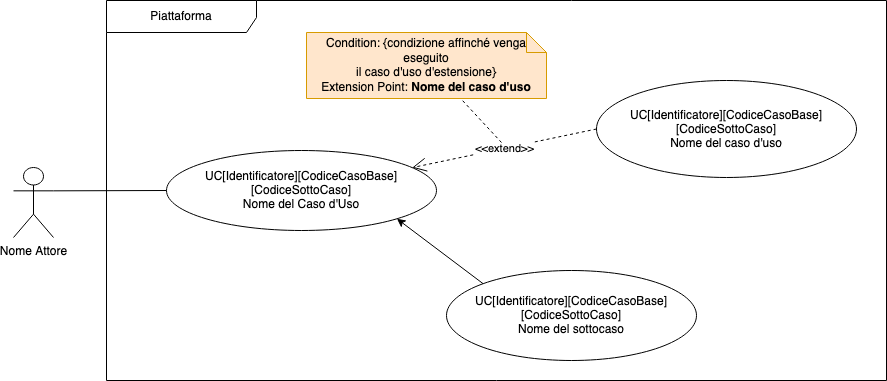
\includegraphics[scale=0.5]{Contenuto/Immagini/UseCase.png}
\caption{Esempio di Caso D'Uso}
\end{figure}

\paragraph{Classificazione requisiti}

Un requisito è un obiettivo, accordato con il proponente o preso mediante una decisione interna, da raggiungere per risolvere un determinato problema. Per rappresentare un requisito, è stato scelto di adottare la seguente convenzione:

\begin{center}
\textbf{R[Importanza][Tipologia][Codice]}
\end{center}

dove:

\begin{itemize}
\item \textbf{Importanza}: rappresenta l'importanza associata al requisito e può assumere uno dei seguenti valori:
\begin{itemize}
	
	\item \textbf{1}: Requisito \textit{Obbligatorio}, la sua soddisfazione dovrà necessariamente avvenire per garantire una buona funzionalità dell’intero sistema;
	\item \textbf{2}: Requisito \textit{Desiderabile}, la sua soddisfazione non vincola il buon funzionamento del sistema, tuttavia ne fornisce una maggior completezza;
	\item \textbf{3}: Requisito \textit{Facoltativo}, se soddisfatto rende il sistema più completo, ma ciò potrebbe comportare un dispendio di energie con un conseguente aumento dei costi preventivati.
\end{itemize}
\item \textbf{Tipologia}: si riferisce alla tipologia di requisito e può assumere uno dei seguenti valori letterali:
\begin{itemize}
	\item \textbf{V}: requisito di \textit{Vincolo}, descrive i vincoli offerti dal sistema;
	\item \textbf{F}: requisito \textit{Funzionale}, descrive servizi o funzioni offerti dal sistema;
	\item \textbf{P}: requisito \textit{Prestazionale}, descrive i vincoli sulle prestazioni da soddisfare, con il numero di informazioni da manipolare in un certo intervallo di tempo;
	\item \textbf{Q}: requisito di \textit{Qualità}, descrive i vincoli di qualità da realizzare.
\end{itemize}
\item \textbf{Codice}: identifica in maniera univoca il requisito in forma gerarchica padre/figlio.
Per esplicitare la forma gerarchica, il codice viene rappresentato come segue:
\begin{center}
\textbf{[Identificatore][CodiceBase](.[CodiceSottoCaso])}
\end{center}
dove: 
\begin{itemize}
	\item \textbf{Identificatore}: può essere presente o meno. Nel caso sia presente, può assumere una delle seguenti espressioni letterali:
		\begin{itemize}
			\item \textbf{W}: identifica un caso d'uso relativo alla WebApp;
			\item \textbf{E}: identifica un caso d'uso di un errore.
		\end{itemize}
	\item \textbf{CodiceBase}: fa riferimento al caso d’uso preso in esame e, in combinazione con la Tipologia, definisce un identificatore univoco per il requisito;
	\item \textbf{CodiceSottoCaso}: codice progressivo opzionale, che può includere più livelli, ed identifica un eventuale sottocaso.
\end{itemize}
\end{itemize}

Dopo aver classificato ciascun requisito con un codice, quest’ultimo non potrà più essere cambiato.
Inoltre, ciascun codice verrà accompagnato da una serie di informazioni aggiuntive, che meglio definiranno ciascun requisito, ossia:

\begin{itemize}
	\item \textbf{Descrizione}: breve descrizione completa relativa allo scopo del requisito;
	\item \textbf{Classificazione}: indica l’importanza del requisito e può assumere i valori \textit{Obbligatorio}, \textit{Desiderabile} e \textit{Facoltativo}. Sebbene questa informazione possa sembrare ridondante, ne facilita la lettura;
	\item \textbf{Fonti}: indica le fonti del requisito, ossia possono essere:
	\begin{itemize}
		\item all'interno del Capitolato d’Appalto;
		\item nei Verbali Interni;
		\item nei Verbali Esterni;
		\item nei Casi d’Uso presenti nel documento “\AdR”;
		\item una decisione presa internamente (quindi “Decisione Interna”).
	\end{itemize}	 
\end{itemize}

Ad esempio:\\
\definecolor{darkblue}{cmyk}{99, 99, 0, 71}

\begin{table}[!htbp]
\renewcommand{\arraystretch}{1.5}
\begin{tabular}{ m{0.15\textwidth}<{\centering}  m{0.37\textwidth}<{\centering}  m{0.23\textwidth}<{\centering}  m{0.15\textwidth}<{\centering}}
    \rowcolor{darkblue}
    \textcolor{white}{\textbf{Requisito}} &\textcolor{white}{\textbf{Descrizione}}& \textcolor{white}{\textbf{Classificazione}} & \textcolor{white}{\textbf{Fonti}}\\ 

    \rowcolor{gray!25} R1FW1 & L’utente deve riuscire ad inserire i propri dati personali (nome, cognome, indirizzo e-mail e password) per effettuare la registrazione & Obbligatorio & UCW1 \\

\end{tabular}
\end{table}

\paragraph{Qualità dei requisiti}
Ciascun requisito deve essere:
\begin{itemize}
  \item Completo, ovvero dettagliato;
  \item Consistente, che non sia in contraddizione con altri requisiti;
  \item Necessario;
  \item Verificabile, ovvero che sia possibile controllare che il sistema lo realizzi;
  \item Tracciabile.
\end{itemize}

\paragraph{Metriche}
Le metriche utilizzate per la valutazione dell'attività di analisi dei requisiti sono:
\begin{itemize}
\item \textbf{MQP05 Percentuale requisiti obbligatori soddisfatti} \\
Indica la quantità percentuale dei requisiti obbligatori soddisfatti in rapporto al totale dei requisiti obbligatori.
La formula è:
\begin{itemize}
  \item[] \[RS = \frac{ROS}{TRO} * 100;\]
  \item RS = Percentuale requisiti obbligatori soddisfatti;
  \item ROS = Requisiti obbligatori soddisfatti;
  \item TRO = Totale requisiti 	obbligatori.
  \end{itemize}
\end{itemize}


\subsubsection{Progettazione}
\paragraph{Scopo}
Lo scopo della Progettazione è di determinare le caratteristiche che il prodotto deve avere per soddisfare i requisiti individuati dagli stakeholder\textsuperscript{G}. Il procedimento seguito è l'opposto rispetto a quello usato per l'\AdR. Vengono individuate le diverse parti, coerenti con i requisiti, che verranno poi raggruppate in vari sottoinsiemi fino ad arrivare ad un'unica soluzione finale. Restano da rispettare i vincoli di sostenibilità nell'utilizzo delle risorse, nel contenimento dei costi e nel rispetto degli obiettivi di qualità.

\paragraph{Descrizione}
L’obiettivo è la realizzazione dell’architettura del sistema.

\paragraph{Technology Baseline}
Misura la comprensione delle tecnologie individuate per la realizzazione del prodotto, motivandone la scelta. 
Dovranno essere mostrate:
\begin{itemize}
	\item Le varie tecnologie adottate, motivando le scelte;
	\item Le relazioni tra i vari componenti e come interagiscono tra di loro;
	\item Il \textit{\textbf{Proof of Concept}}: un prototipo (incompleto) eseguibile che riunisce tutte le tecnologie adottate, dimostrando in maniera pratica la loro adeguatezza e compatibilità reciproca. 
\end{itemize}

\paragraph{Product Baseline}
Rappresenta la baseline architetturale (design e coding) del prodotto, coerente con la Technology Baseline. Mostra il design definitivo del prodotto.
Dovrà contenere:
\begin{itemize}
	\item Diagrammi UML delle classi e di sequenza;
	\item Tracciamento per ogni classe dei requisiti che deve soddisfare;
	\item Descrizione dei design pattern utilizzati;
	\item Descrizione dell'architettura generale del prodotto software.
\end{itemize}

\paragraph{Qualità}
È compito del \textit{Progettista} definire un'architettura di qualità. Le caratteristiche che essa dovrà avere sono:

\begin{itemize}
  \item Soddisfare i requisiti indicati nel documento \AdR;
  \item Essere comprensibile, robusta e affidabile;
  \item Presentare componenti semplici, in maniera tale da garantire modularità e riusabilità, semplificando il lavoro dello sviluppatore;  
  \item Utilizzare le risorse in maniera efficiente.
\end{itemize}


\subsubsection{Codifica}
\paragraph{Scopo}
Lo scopo del processo di codifica è l'effettiva realizzazione del prodotto software, svolto dal \textit{\PR}. Si può vedere come la trasformazione in codice dell’architettura definita dai \textit{Progettisti}, per arrivare allo sviluppo del prodotto finale.

\paragraph{Descrizione}
Il codice deve rispettare gli obiettivi di qualità definiti nel \PdQ. Nelle sezioni sottostanti saranno elencate regole e norme di carattere più generale, utilizzate da ogni linguaggio di programmazione impiegato nel progetto. 

\paragraph{Stile di codifica}

\subparagraph{Norme di buona programmazione}
Di seguito le più importanti norme guida generali per lo sviluppo del codice che il gruppo si impegna a rispettare: 
\begin{itemize}
\item Produrre codice leggibile e verificabile;
\item Strutturare la codifica in modo da rispettare il design progettato;
\item Massimizzare l'information hiding.
\end{itemize}

\subparagraph{Brevità dei metodi}
In generale ogni metodo o procedura dovrebbe essere breve e conciso, tra le 20 e 25 righe (contando un'istruzione per riga). Poiché il bisogno di scrivere un metodo più lungo può diventare necessario, si possono considerare tollerabili procedure fino ad un massimo di 35-40 righe. Nel caso in cui la soglia venga superata, ha senso considerare una suddivisione della procedura. E' fondamentale concentrarsi sullo scopo di ogni procedura, evitando singole procedure che svolgono troppi compiti.

\subparagraph{Norme di struttura per il linguaggio Python}
Molte di queste norme derivano dallo standard di codifica Python PEP 8 che il gruppo di sviluppo della parte di backend si impegna a rispettare.
\begin{itemize}
\item \textbf{Indentazione}: i blocchi di codice innestati dovranno avere un’indentazione di quattro spazi, evitando l'utilizzo di tabulazioni;
\item \textbf{Lunghezza massima}: Ogni riga di codice dovrà avere una lunghezza massima di 79 caratteri; 
\item \textbf{Import}: Ogni import vanno generalmente in linee separate (da evitare import multipli separati da virgola), e vanno raggruppati per categorie (librerie standard, librerie di terze parti, librerie specifiche dell'applicazione) separate da una linea vuota;
\item \textbf{Commenti}: i commenti al codice saranno presentati in lingua inglese. Se necessari dovranno trovarsi generalmente sopra al costrutto in questione;
\item  \textbf{Univocità dei nomi}: tutti i costrutti dovranno avere nomi univoci ed autoesplicativi, da evitare nomi eccessivamente lunghi.
\item \textbf{Operazioni logiche/matematiche}: Preferibilmente vanno spezzate portanto il simbolo dell'operazione (es. "+") nella nuova linea.
\end{itemize}

\subparagraph{Convenzioni sulla nomenclatura per il linguaggio Python}
Molte di queste norme derivano dallo standard di codifica Python PEP 8 che il gruppo di sviluppo della parte di backend si impegna a rispettare.

In generale per i nomi verrà utilizzata la nomenclatura "snake case", dove ogni parola è in minuscolo, separata da un underscore, con alcune particolarità:
\begin{itemize}
\item Nomi di variabili e metodi dovranno cominciare con la lettera minuscola;
\item Nomi di classi e file dovranno cominciare con la lettera maiuscola e rispettare la convenzione camel case, dove le parole sono unite tra di loro e l'iniziale di ogni parola è in maiuscolo;
\item Nomi di costanti dovranno essere scritti tutti in maiuscolo, separando le parole con il carattere underscore "\_" ;
\item I nomi delle varie cartelle e package dovranno essere il snake case, con le iniziali minuscole e vanno preferiti nomi brevi e composti da una singola parola.
\end{itemize}

\subparagraph{Norme di struttura per il linguaggio Javascript}

\begin{itemize}
\item robe
\end{itemize}

\subparagraph{Convenzioni sulla nomenclatura per il linguaggio Javascript}

\begin{itemize}
\item robe
\end{itemize}


\paragraph{Metriche}
Per la valutazione del processo di codifica saranno adottate le seguenti metriche:
\begin{itemize}

\item \textbf{MQP02 Profondità di una gerarchia} \\
È un valore intero che definisce quanto può essere profonda la gerarchia di una classe. Nel caso una gerarchia abbia una sola classe, allora il suo valore sarà pari a 1;

\item \textbf{MQP03 Numero parametri per metodo} \\
Indica il numero intero di parametri che può avere un metodo. Un numero di parametri troppo elevato, indica che è necessario ridurre delle funzionalità associate al metodo a cui si fa riferimento. Inoltre, se si ha un numero elevato di parametri, la probabilità di avere più errori progettuali aumenta;

\item \textbf{MQP05 Percentuale requisiti obbligatori soddisfatti} \\
Indica la quantità percentuale dei requisiti obbligatori soddisfatti in rapporto al totale dei requisiti obbligatori.
La formula è:
\begin{itemize}
  \item[] \[RS = \frac{ROS}{TRO} * 100;\]
  \item RS = Percentuale requisiti obbligatori soddisfatti;
  \item ROS = Requisiti obbligatori soddisfatti;
  \item TRO = Totale requisiti 	obbligatori.
  \end{itemize}

\item \textbf{MQP06 Complessità ciclomatica}\\
La complessità ciclomatica è una metrica sviluppata da Thomas J. McCabeornisce che fornisce una misura quantitativa della complessità di un programma, essa è identificata dal numero di cammini linearmente indipendenti presenti nel grafo del flusso di controllo del programma. Un valore elevato di tale misurazione indica che il software possiede un comportamento poco predicibile, fattore che causa grandi rischi.
La formula è:
\begin{itemize}
  \item[] \[CC 	= E - N + P;\]
  \item CC = Complessità ciclomatica;
  \item E = Numero di congiunzioni tra statement (gli archi di un grafo);
  \item N = Numero di statement (nodi presenti nel grafo);
  \item P = Numero delle componenti connesse da ogni nodo (per esecuzione sequenziale P = 2 essendovi 1 predecessore e 1 successore per ogni arco).
  \end{itemize}


\item \textbf{MQP07 Numero di bug}\\
Numero di righe di codice del programma che potrebbero comportare un risultato diverso da quello previsto.

\item \textbf{MQP08 Numero di code smell}\\
Indica una serie di caratteristiche che il codice sorgente può avere e che sono generalmente riconosciute come probabili indicazioni di un difetto di programmazione.

\item \textbf{MQP09 Linee di Commento per Linee di Codice} \\
La formula è:
\begin{itemize}
  \item[] \[LCC = \frac{LDC}{LCD} * 100 ;\]
  \item LCC = Percentuale rapporto tra linee di commento e linee di codice di istruzioni;
  \item LDC = Linee di commento;
  \item LCD = Linee di codice.
  \end{itemize}


\item \textbf{MQP12 Numero di vulnerabilità}\\
Indica il numero di vulnerabilità presenti nel codice sorgente del prodotto.
\end{itemize}
Per maggiori informazioni consultare \S{}C.

\paragraph{Strumenti}
Gli strumenti che verranno adottati durante il processo di sviluppo sono:
\begin{itemize}
\item \textbf{PyCharm Community Edition}: IDE preferito per lo sviluppo in Python, per il fatto che offre uno strumento nativo di refactor automatico che impone il rispetto dello standard PEP 8.
\item \textbf{Atom}: IDE preferito per lo sviluppo in Javascript/HTML/CSS;
\item \textbf{Visual Studio Code}: IDE alternativo utilizzato dal gruppo per la stesura del codice;
\item \textbf{AWS CLI}\textsuperscript{G}: uno strumento unificato per la gestione dei servizi AWS\textsuperscript{G} via interfaccia a riga di comando.
\item \textbf{StarUML}: strumento utilizzato per la produzione dei diagrammi UML.

\end{itemize}

	\pagebreak
	\section{Processi di Supporto}
\subsection{Documentazione}
\subsubsection{Scopo}
Ogni processo e attività per lo sviluppo del progetto dovrà essere documentata. Nella presente sezione verranno descritte regole e standard da seguire durante il processo di documentazione per l'intero ciclo di vita\textsuperscript{G} del software.

\subsubsection{Descrizione}
Vengono presentate decisioni e norme prescelte per:
\begin{itemize}
  \item Stesura;
  \item Verifica;
  \item Approvazione.
\end{itemize}

\subsubsection{Documenti prodotti}
I documenti prodotti sono:
\begin{itemize}
  \item \textbf{Norme di progetto}: documento interno che contiene norme e regole stabilite dal gruppo, che devono essere seguite per l’intera durata del progetto;
  \item \textbf{Glossario}: documento esterno dove sono presenti i termini tecnici usati nella documentazione con le loro definizioni, affinché non ci siano ambiguità e/o incongruenze;
  \item \textbf{Piano di progetto}: documento esterno con la pianificazione delle attività del progetto previste dal gruppo. Contiene la previsione dell’impegno orario dei singoli membri, il preventivo spese e i consuntivi di periodo;
  \item \textbf{Piano di qualifica}: documento esterno che descrive i criteri con cui si valuta la qualità;
  \item \textbf{Analisi dei requisiti}: documento esterno contenente requisiti e caratteristiche del prodotto finale;
  \item \textbf{Verbali}:
  \begin{itemize}
  		\item Interni: resoconti degli incontri del gruppo;
  		\item Esterni: resoconti degli incontri del gruppo con i committenti e/o il proponente.
	\end{itemize}
\end{itemize}

\subsubsection{Sistema software per la preparazione dei documenti}
Tutti i documenti prodotti dal gruppo verranno redatti usando il linguaggio di markup \LaTeX.

\subsubsection{Ciclo di vita di un documento}
Ogni documento passa per i seguenti step:
\begin{itemize}
  \item \textbf{Creazione}: il documento viene creato basandosi su un template comune;
  \item \textbf{Strutturazione}: il documento viene fornito di:
  \begin{itemize}
  		\item Registro delle modifiche;
  		\item Indice dei contenuti.
	\end{itemize}
  \item \textbf{Stesura}: il gruppo redige il documento adottando il metodo incrementale;
  \item \textbf{Revisione}: ogni sezione del corpo del documento è rivista da almeno un membro del gruppo che non sia il redattore della parte in verifica;
  \item \textbf{Approvazione}: se revisionato, il Responsabile di Progetto può stabilire che il documento è valido. Se approvato, può essere rilasciato.
\end{itemize}
Per semplificare le operazioni di verifica dovrà sempre essere reso disponibile il documento  completo (fino alla versione più attuale) in formato PDF.

\subsubsection{Struttura delle directory e dei files}
Per ogni documento si definisce la seguente struttura di directory:\\
\begin{forest}
  for tree={
    font=\ttfamily,
    grow'=0,
    child anchor=west,
    parent anchor=south,
    anchor=west,
    calign=first,
    edge path={
      \noexpand\path [draw, \forestoption{edge}]
      (!u.south west) +(7.5pt,0) |- node[fill,inner sep=1.25pt] {} (.child anchor)\forestoption{edge label};
    },
    before typesetting nodes={
      if n=1
        {insert before={[,phantom]}}
        {}
    },
    fit=band,
    before computing xy={l=15pt},
  }
[NomeDocumento
  [NomeDocumento.tex]
  [NomeDocumento.pdf]
  [Contenuto
    [Sezioni
        [Introduzione.tex]
        [Sezione1.tex]
        [Sezione2.tex]
    ]
    [Immagini
        [Immagine1.png]
        [Immagine2.jpeg]
    ]
    [Intro.tex]
    [RegistroModifiche.tex]
  ]
  [Struttura
    [Command.tex]
    [Impaginazione.tex]
    [Packages.tex]
  ]
]
\end{forest}\\

In particolare:
\begin{itemize}
\item \textbf{NomeDocumento.tex}: importa tutti le parti necessarie per comporre il documento finale;
\item \textbf{NomeDocumento.pdf}: versione del documento in formato PDF;
\item \textbf{Introduzione.tex}:  sezione introduttiva del documento, definisce lo scopo del prodotto e del documento, i riferimenti normativi e informativi e informazioni sul \textit{Glossario};
\item \textbf{Intro.tex}: contiene tutti i comandi per creare la prima pagina del documento;
\item \textbf{RegistroModifiche.tex}: contiene tutti i comandi per creare la tabella del registro delle modifiche;
\item \textbf{Command.tex}: contiene tutti i comandi aggiuntivi creati dal gruppo;
\item \textbf{Impaginazione.tex}: definisce alcune istruzioni per l'impaginazione e si occupa di creare header e footer del documento;
\item \textbf{Packages.tex}: contiene tutti i pacchetti aggiuntivi e necessari per la compilazione.
\end{itemize}


\subsubsection{Struttura di un documento}
\paragraph{Prima pagina}
La prima pagina è composta da:
\begin{itemize}
  \item \textbf{Logo del gruppo};
  \item \textbf{Titolo del documento};
  \item \textbf{Informazioni varie del documento}:
      \begin{itemize}
      \item \textbf{Versione corrente};
      \item \textbf{Approvatori}: indica chi ha approvato il documento. Se non presente, indica che il documento non è ancora stato approvato;
      \item \textbf{Data approvazione};
      \item \textbf{Redattori}: indica chi si è occupato della stesura del documento;
      \item \textbf{Verificatori}: indica chi si è occupato della verifica del documento;
      \item \textbf{Uso}: indica se il documento è dedicato a uso interno o esterno;
      \item \textbf{Distribuzione}: indica a chi viene distribuito il documento;
        \end{itemize}
\item \textbf{Indirizzo e-mail del gruppo}.
\end{itemize}

\paragraph{Registro delle modifiche}
Ogni documento ha il suo registro modifiche che tiene traccia di tutte le modifiche importanti del documento durante il suo ciclo di vita.
Sotto forma di tabella, riporta:
  \begin{itemize}
  		\item Versione del documento dopo la modifica;
  		\item Data della modifica;
  		\item Nome dell’autore della modifica;
  		\item Ruolo dell’autore al momento della modifica;
  		\item Descrizione breve della modifica;
  		\item Nome della persona che si è occupata di verificare la modifica.
	\end{itemize}

Inoltre, nella descrizione di ciascuna modifica viene indicato anche il paragrafo interessato con questa convenzione: 
\begin{itemize}
    \item \textbf{\S{}}: indica un solo paragrafo;
    \item \textbf{\S{}\S{}}: indica l'intervallo di paragrafi su cui sono state apportate le modifiche fatte.
\end{itemize}

\paragraph{Indice}
Presente dopo il registro delle modifiche, l’indice permette di avere una visione completa del documento e di individuare le varie parti, ogni voce è un collegamento ipertestuale alla parte del documento in cui viene trattata.

\paragraph{Struttura delle pagine}
Ogni pagina, a eccezione della prima, è formata da questi elementi:
  \begin{itemize}
  		\item In alto a sinistra si trova una miniatura a colori del logo del gruppo;
  		\item In alto a destra è presente il titolo del documento;
  		\item Sotto i due elementi appena elencati una linea nera continua li separa dal contenuto della pagina;
  		\item Il contenuto della pagina;
  		\item Sul lato destro del piè di pagina è indicato il numero della pagina corrente.
	\end{itemize}
	
\paragraph{Verbali}
I verbali applicano le stesse norme strutturali degli altri documenti con la differenza che non sono soggetti a versionamento\textsuperscript{G}. Ogni verbale sia interno che esterno dovrà contenere:
\begin{itemize}
\item Motivo della riunione;
\item Luogo della riunione;
\item Data della riunione;
\item Orario di inizio e fine riunione;
\item Partecipanti della riunione;
\item Resoconto della riunione;
\item Registro delle decisioni, dove si riporta in tabella le decisioni prese dal gruppo durante l’incontro.
\end{itemize}  		

\subsubsection{Normativa tipografica}
\paragraph{Nomi dei documenti}
La struttura generale del nome è la seguente: \\ \\
\centerline{\textbf{[NomeDocumento]-v[X].[Y].[Z]}}\\
in particolare:
\begin{itemize}
\item \textbf{[NomeDocumento]} inizia sempre con la lettera maiuscola. Se presenti più parole, queste saranno attaccate ma distinguibili dalla lettera maiuscola (convenzione \textit{"CamelCase"}\textsuperscript{G});
\item \textbf{v[X].[Y].[Z]} rappresenta la versione corrente del documento seguendo lo schema di versionamento presentato in §3.2.3;
\end{itemize}
I verbali, in quanto non soggetti a versionamento avranno una struttura del nome diversa, ovvero:\\ \\
\centerline{\textbf{Verbale[Tipologia]-[YYYY].[MM].[DD]}} \\
dove:
\begin{itemize}
\item \textbf{[Tipologia]} intende il tipo del verbale, può essere \textbf{Interno} o \textbf{Esterno};
\item \textbf{[YYYY].[MM].[DD]} indica la data in cui è avvenuto l'incontro.
\end{itemize}


\paragraph{Stile di testo}
Gli stili di testi adottati nei documenti sono:
\begin{itemize}
\item \textbf{Grassetto}: per titoli, sottotitoli, e altri termini ritenuti importanti dal redattore;
\item \textbf{Maiuscolo}: per acronimi e iniziali di nomi propri, dei documenti o dei paragrafi;
\item \textbf{Corsivo}: per nomi propri dei membri del gruppo, committenti e proponente e per i nomi dei documenti.
\end{itemize}


\paragraph{Termini di glossario}
I termini che possono risultare ambigui e/o incongruenti sono contrassegnati con una \textsuperscript{G} alla loro prima occorrenza nella sezione d’interesse. Questi termini sono riportati con il loro significato in un documento esterno, il \textit{Glossario}.

\paragraph{Elementi testuali}
I redattori devono seguire le seguenti regole stilistiche:
\begin{itemize}
\item \textbf{Elenchi puntati}: un elenco puntato utilizzerà il simbolo • (pallino). Un successivo annidamento utilizzerà il simbolo - (trattino) e un altro ancora un asterisco (*). Se si tratta di un elenco numerato, i quattro livelli di enumerazione sono ordinati con i numeri arabi divisi da un punto fermo. Ogni voce dell’elenco inizia con una lettera maiuscola e termina con un punto e virgola, tranne l'ultima voce che termina con un punto;

\item \textbf{Formati di data}: Le date usano il formato \textbf{[YYYY]-[MM]-[DD]} dove:
    \begin{itemize}
    \item \textbf{[YYYY]} corrisponde all’anno;
    \item \textbf{[MM]} corrisponde al mese;
    \item \textbf{[DD]} corrisponde al giorno.
    \end{itemize}

\item \textbf{Orario}: gli orari usano il formato \textbf{[HH]:[MM]} dove:
    \begin{itemize}
    \item \textbf{[HH]} rappresentano le ore;
    \item \textbf{[MM]} rappresentano i minuti.
    \end{itemize}

\item \textbf{Sigle}: Tutte le sigle hanno le iniziali di ogni parola maiuscola tranne preposizioni, congiunzioni e articoli. Le sigle utilizzate sono:
    \begin{itemize}
    \item Relative ai documenti:
        \begin{itemize}
        \item \textbf{Analisi dei Requisiti}: AdR;
        \item \textbf{Piano di Progetto}: PdP;
        \item \textbf{Piano di Qualifica}: PdQ;
        \item \textbf{Glossario}: G;
        \item \textbf{Norme di Progetto}: NdP;
        \item \textbf{Verbali Interni}: VI;
        \item \textbf{Verbali Esterni}: VE.
        \end{itemize}
    
    \item Relative ai ruoli di progetto:
        \begin{itemize}
        \item \textbf{Responsabile di Progetto}: RE;
        \item \textbf{Progettista}: PT;
        \item \textbf{Analista}: AN;
        \item \textbf{Amministratore}: AM;
        \item \textbf{Programmatore}: PR;
        \item \textbf{Verificatore}: VE.
        \end{itemize}
    \end{itemize}
\end{itemize}

\paragraph{Elementi grafici}
Le regole per quanto riguarda l’uso di elementi grafici sono:
\begin{itemize}
\item \textbf{Immagini}: le figure presenti sono centrate rispetto al testo e accompagnate da didascalia;
\item \textbf{Diagrammi UML}: verranno inseriti nel documento tramite delle immagini.
\end{itemize}

\subsubsection{Metriche}
Per la valutazione dei documenti prodotti del processo di documentazione, verrà applicata la seguente metrica di prodotto:
\begin{itemize}
\item \textbf{MQP01 Indice di Gulpease}, trattato nell'appendice C.1. 
\end{itemize}

\subsubsection{Strumenti}
Gli strumenti dedicati alla stesura sono:
\begin{itemize}
\item \textbf{\LaTeX}: linguaggio compilato basato sul programma di composizione tipografica Tex;
\item \textbf{Texmaker}: l’editor per la stesura dei documenti;
\item \textbf{Overleaf}: editor per la stesura dei documenti basato sul cloud\textsuperscript{G} ;
\item \textbf{Draw.io}: sito online per la creazione di grafici UML;
\item \textbf{GanttProject}: programma usato per la realizzazione di diagrammi di Gantt\textsuperscript{G}.
\end{itemize}

\subsection{Gestione della configurazione}
\subsubsection{Scopo}
Lo scopo è di gestire e controllare la produzione di documenti e codice in maniera sistematica. Per ogni oggetto sottoposto a configurazione viene garantito il versionamento e controllo sulle modifiche per permettere il mantenimento dell'integrità del prodotto. 

\subsubsection{Descrizione}
Vengono raggruppati e organizzati tutti i mezzi usati per la configurazione degli strumenti designati alla produzione di documenti e codice, per poter gestire struttura e la disposizione dei file all’interno del repository\textsuperscript{G} e anche  quelli per versionamento e coordinamento.

\subsubsection{Versionamento}
Per poter capire lo stato di avanzamento di un prodotto delle attività del progetto è necessario un identificatore. Il formato del codice di versione utilizzato è \\ \\
\centerline{\textbf{v[X].[Y].[Z]}} \\ \\
dove :
\begin{itemize}
\item \textbf{X} indica il rilascio pubblico e corrisponde ad una versione approvata dal Responsabile di Progetto. La numerazione parte da 0;
\item \textbf{Y} indica una revisione complessiva del prodotto per verificare che, dopo una modifica, il prodotto sia ancora coeso e consistente. La numerazione parte da 0 e si azzera ad ogni incremento di X;
\item \textbf{Z} viene incrementato ad ogni modifica con relativa verifica. La numerazione parte da 0 e si azzera ad ogni incremento di X o Y.
\end{itemize}

\paragraph{Strumenti}
Per il versionamento si è scelto di utilizzare un repository GitHub, che, a sua volta, implementa il software di controllo versione distribuito Git.

\subsubsection{Struttura del repository}
Il repository utilizzato dal gruppo per la creazione dei documenti contiene una directory per ogni documento denominata NomeDocumento, la cui struttura è approfondita in §3.1.6.
Il repository è suddiviso in più branch così definiti:
\begin{itemize}
\item \textbf{main}: il branch principale, che contiene l'ultima versione verificata di ogni documento;
\item \textbf{NomeDocumento}: uno per ogni documento, è dove il documento vive e viene attivamente stilato dai membri del gruppo.
\end{itemize}

\subsubsection{Modifiche al repository}
Non è consentito fare commit\textsuperscript{G} direttamente sul branch\textsuperscript{G} \textbf{main}, poiché porterebbe ad un elevato rischio di incongruenze e merge conflicts\textsuperscript{G}. Potrà essere modificato solo tramite il meccanismo di pull request\textsuperscript{G} con verifica obbligatoria, in modo da garantire che sia sempre presente una versione verificata e corretta del documento, anche se incompleta.
Nel branch \textbf{NomeDocumento} invece ogni membro può fare commit a patto che siano relative solo al documento specificato. Ogni commit deve referenziare la issue\textsuperscript{G} da cui è derivata e quindi, in generale, potranno effettuare modifiche sul branch solo gli assegnatari di issue che trattano quel documento specifico. Per quanto riguarda cambiamenti minimali (punteggiatura, errori ortografici, ecc.) è permessa la modifica autonoma da parte di qualsiasi membro del gruppo e non è necessario referenziare nessuna issue.
La gestione delle issue (ticket) viene trattata in §4.1.4.2.

\subsection{Gestione della qualità}
\subsubsection{Scopo}
Lo scopo del processo di gestione della qualità è di assicurare che i requisiti di qualità individuati dagli stakeholder e le esigenze espresse dal proponente vengano rispettate dai prodotti e processi da sviluppare.

\subsubsection{Descrizione}
Il \textit{Piano di Qualifica} è il documento dedicato alla gestione della qualità. In esso sono descritti metriche e standard con le quali misurare e valutare la qualità di prodotti e processi.  

\subsubsection{Attività di processo}
Si possono individuare tre attività principali nel processo di gestione della qualità:
\begin{itemize}
\item \textbf{Pianificazione}: definire obiettivi di qualità, le strategie per raggiungerli e le risorse necessarie; 
\item \textbf{Valutazione}: applicare quanto pianificato, misurando i risultati;
\item \textbf{Reazione}: analizzando i risultati ottenuti con lo scopo di attuare miglioramenti o sanare situazioni non desiderate.
\end{itemize}

\subsubsection{Controllo di qualità}
Per essere sicuri di arrivare alla qualità desiderata, ogni membro deve essere in grado di:
\begin{itemize}
\item Comprendere gli obiettivi da raggiungere;
\item Individuare eventuali errori;
\item Stimare in termini di valore, dimensione e complessità le task;
\item Produrre risultati concreti e quantificabili.
\end{itemize}

\subsubsection{Denominazione metriche e obiettivi}
Per la denominazione delle metriche è stato adottato il formato: \\ \\
\centerline{\textbf{M[Tipologia][Numero]}} \\ \\
mentre per la denominazione degli obiettivi di qualità è stato adottato il formato: \\ \\
\centerline{\textbf{Q[Tipologia][Numero]}} \\ \\
dove:
\begin{itemize}
\item \textbf{[Tipologia]}: indica la tipologia a cui si riferisce la metrica, può assumere tre valori:
    \begin{itemize}
    \item \textbf{PC}: relativa ai processi; 
    \item \textbf{QP}: relativa ai prodotti;
    \item \textbf{TS}: relativa ai test.
    \end{itemize}
\item \textbf{[Numero]}: indica il numero progressivo della metrica, parte da 1.
\end{itemize}	

\subsection{Verifica}
\subsubsection{Scopo}
Lo scopo è definire come attuare il processo di verifica, per accertarsi che non ci siano errori durante lo sviluppo del prodotto, che la redazione della documentazione e che i requisiti in oggetto vengano rispettati. 

\subsubsection{Descrizione}
La verifica viene applicata ad ogni processo in esecuzione. Per il processo di verifica ci si affida all'analisi e ai test. L'analisi si divide in due tipologie:
\begin{itemize}
\item \textbf{Statica}: non richiede l'esecuzione dell'oggetto in verifica, perciò è applicabile ad ogni prodotto. Accerta il rispetto della normativa e l'assenza di errori studiando il codice sorgente o la documentazione;
\item \textbf{Dinamica}: richiede l'esecuzione dell'oggetto in verifica, applicabile perciò solo al codice. Fa largo uso di test.
\end{itemize}

\subsubsection{Verifica della documentazione}
Si utilizza un'analisi statica. Si possono utilizzare strumenti automatici oppure si può fare a mano (desk check) attraverso due metodi:
\begin{itemize}
\item \textbf{Walkthrough}: che consiste in un controllo completo del documento tramite una lettura ad ampio spettro;
\item \textbf{Inspection}: che consiste in un controllo specifico tramite una lettura mirata del documento.
\end{itemize}

\paragraph{Walkthrough}
Attività svolta dal \VE{}, viene di norma adottata nelle fasi iniziali. Risulta essere molto onerosa e quindi va ridotto l'uso il prima possibile. Nel caso del nostro gruppo, questo metodo verrà adottato fino a che non sarà disponibile una lista di controllo.

\paragraph{Inspection}
Attività svolta dal \VE{}, sfrutta una lettura mirata per trovare gli errori tramite una lista di controllo, compilata seguendo gli errori più comuni nelle varie verifiche in modalità Walkthrough. Rispetto la tecnica Walkthrough, questo metodo è meno oneroso e da preferire, verrà utilizzato dal nostro gruppo quando sarà disponibile una lista di controllo esaustiva.


\subsubsection{Verifica del codice}
Si utilizza sia l'analisi statica che quella dinamica. In particolare con:
\begin{itemize}
\item L'analisi statica si controlla la bontà del codice, sia dal punto di vista della correttezza che del rispetto delle norme di buona programmazione definite dal gruppo (vedi §2.4.3.1);
\item L'analisi dinamica si controlla la presenza o meno di bug durante l'esecuzione del software prodotto.
\end{itemize}

\paragraph{Test}
I test sono l'attività fondamentale dell'analisi dinamica. Servono per dimostrare che il programma funzioni e svolga ciò per cui è stato sviluppato. I test si dividono in quattro categorie, in base all'oggetto in verifica e allo scopo: 
\begin{itemize}
\item \textbf{Test d'unità}: verificano una singola unità di codice, la più piccola parte che ha senso verificare (es. singola procedura);
\item \textbf{Test d'integrazione}: verificano la correttezza delle interfacce. Si vuole stabilire il corretto funzionamento delle varie componenti, una volta passato il test d'unità, aggregandole man mano e verificando il funzionamento nel complesso;
\item \textbf{Test di sistema}: verifica l'applicazione nella sua interezza. Venendo dopo il test d'integrazione, lo scopo è verificare che le componenti non solo sono compatibili, ma che lo scambio di dati tra interfacce e le varie interazioni siano conformi. Inoltre, così si controlla che i requisiti siano stati soddisfatti;
\item \textbf{Test di regressione}: verifica l'applicazione dopo aver apportato modifiche al sistema. Lo scopo è controllare nuove funzionalità non testate e, al tempo stesso, garantire che il codice già presente e testato in precedenza non subisca alterazioni al suo comportamento.
\end{itemize}

\paragraph{Nominazione dei test}
Ogni test verrà identificato con un codice: \\ \\
\centerline{\textbf{T[Tipologia][Id]}} \\ \\
In particolare:
\begin{itemize}
\item \textbf{Tipologia}: Indica la tipologia del test:
	\begin{itemize}
	\item \textbf{U}: Unità;
	\item \textbf{I}: Integrazione;
	\item \textbf{S}: Sistema;
	\item \textbf{R}: Regressione.
	\end{itemize}

\item \textbf{Id}: codice numerico per identificare i test dello stesso tipo, parte da 1.

\end{itemize}


\subsubsection{Verifica dei requisiti}
Vengono applicate Walkthrough e Inspection per controllare validità e coerenza con quanto dichiarato e descritto all'interno dell'\textit{Analisi dei Requisiti}, oltre a quanto dichiarato al proponente.

\subsubsection{Metriche}
Per la valutazione del processo di verifica si useranno le seguenti metriche:
\begin{itemize}
\item \textbf{MQP04 Code coverage};
\item \textbf{MQP10 Branch coverage};
\item \textbf{MQP11 Successo dei test}.
\end{itemize}

Per maggiori informazioni consultare l'appendice C.

\subsection{Validazione}
\subsubsection{Scopo}
Lo scopo è stabilire se il prodotto è in grado di soddisfare l'obiettivo per il quale è stato creato. Una validazione con esito positivo certifica che il software soddisfi e sia conforme ai requisiti del proponente.

\subsubsection{Descrizione}
Questo processo avviene dopo il processo di verifica, validando i risultati dei test e garantendo che siano conformi ai requisiti del proponente. Il compito spetta al \RE che controlla i risultati ottenuti e può:
\begin{itemize}
\item Accettare e approvare il prodotto;
\item Rifiutare e chiedere un'ulteriore verifica con delle nuove indicazioni.
\end{itemize}


	\pagebreak
	 \section{Processi Organizzativi}

\subsection{Gestione di processo}

\subsubsection{Scopo}
Secondo lo standard ISO-12207:1995 la gestione di processo contiene le attività e i compiti generici utili per la gestione dei rispettivi processi. Vengono individuate le seguenti attività:
\begin{enumerate}
\item Inizializzazione e definizione dello scopo;
\item Pianificazione e stima dei tempi, delle risorse, dei costi, assegnazione di compiti e responsabilità;
\item Esecuzione e controllo;
\item Revisione e valutazione;
\item Determinazione della fine del processo.
\end{enumerate}

\subsubsection{Obiettivi}
\begin{itemize}
\item Semplificare e gestire la comunicazione tra i membri del gruppo e l'esterno;
\item Coordinare l'assegnazione dei ruoli e compiti;
\item Monitorare il lavoro del gruppo e pianificare le attività da svolgere;
\item Definire le linee guida generali per la formazione dei membri.
\end{itemize}

\subsubsection{Coordinamento}
L'attività di coordinamento è responsabile della gestione delle comunicazioni interne, esterne e delle riunioni.


\paragraph{Comunicazione}
Le comunicazioni avvengono su due piani diversi: tra i membri del gruppo (interno), tra i membri del gruppo e uno o più soggetti esterni (esterno). I soggetti esterni si identificano in:
\begin{itemize}
\item \textbf{Proponente}: l'azienda \textit{\zd};
\item \textbf{Committenti}:  Prof. \textit{Tullio Vardanega} e Prof. \textit{Riccardo Cardin}.
\end{itemize}

\subparagraph{Comunicazione interna}
I principali mezzi di comunicazione tra membri del gruppo sono: Slack\textsuperscript{G} e Telegram\textsuperscript{G}. 
In particolare, per Slack sono stati creati dei canali appositi per argomenti ed i membri del gruppo dovranno intrattenere le discussioni nei canali ritenuti più appropriati, per evitare confusione e/o ammassi incoerenti di messaggi. La creazione dei canali è stata fatta dal Responsabile di Progetto ed essi saranno destinati a mutare nel tempo per accomodare le esigenze del gruppo.
Telegram viene usato per la componente più informale delle discussioni, per le decisioni meno importanti o in caso di problemi con il funzionamento di Slack (da considerarsi comunque una possibilità remota). 

Per quanto riguarda la comunicazione interna tramite videochiamata (tipicamente le riunioni) lo strumento principale è Discord, scelto poiché semplice, conosciuto da tutti i membri del gruppo e multipiattaforma. In alternativa verrà utilizzato Google Meet o Zoom, entrambi strumenti con i quali tutti i membri del gruppo hanno già avuto esperienza.

\subparagraph{Comunicazione esterna}
Per la comunicazione con i soggetti esterni verrà utilizzato un indirizzo e-mail apposito: \textsl{\href{mailto:dreamteam.unipd@gmail.com}{dreamteam.unipd@gmail.com}} .
Tutti i membri del gruppo avranno accesso alla casella di posta elettronica e saranno tenuti a verificare e notificare il gruppo circa la ricezione di nuovi messaggi, mentre la stesura e l'invio di un nuovo messaggio spetterà al Responsabile di Progetto. Prima dell'invio del messaggio, quest'ultimo sarà sottoposto ad una breve verifica e approvazione da parte del gruppo.
Si sono decise le seguenti convenzioni per quanto riguarda la struttura delle e-mail:
\begin{itemize}
\item L'oggetto dovrà terminare con la dicitura "| SWE - Unipd";
\item In generale il corpo dovrà mantenere un tono il più possibile formale ed il contenuto dovrà essere chiaro e conciso;
\item Il corpo dovrà terminare con la firma "\textit{DreamTeam}".
\end{itemize}

\paragraph{Riunioni}
Le riunione potranno essere interne o esterne. Prima di ogni riunione verrà nominato un segretario che ha lo scopo di far rispettare l'ordine del giorno e dirigere la discussione, tenendo traccia dei punti salienti per poi poter redigere il verbale.

\subparagraph{Riunioni interne}
Alle riunioni interne parteciperanno solo i membri del gruppo, per essere considerate valide dovranno essere presenti almeno quattro dei membri del gruppo. Prima di ogni riunione il Responsabile di Progetto dovrà:
\begin{itemize}
\item fissare la data e l'orario;
\item definire l'ordine del giorno;
\item nominare il segretario;
\item comunicare tutto quanto detto sopra (o eventuali variazioni) ai membri con ragionevole anticipo.
\end{itemize}

Gli incontri saranno svolti a cadenza settimanale e, in caso di necessità, anche più frequentemente.
Ogni membro può rivolgersi al Responsabile di progetto per richiedere una riunione interna, proponendo l'ordine del giorno, poi se ritenuta necessaria il Responsabile si attiverà per l'organizzazione dell'incontro.

In ogni caso i membri del gruppo sono liberi di indire riunioni informali tra gli interessati, le persone coinvolte gestiranno orari, date e temi di discussione tra di loro come meglio credono senza intervento del Responsabile di Progetto.
Generalmente la riunione non sarà considerata valida e non sarà prodotto un verbale.

\subparagraph{Riunioni esterne}
Alle riunioni esterne parteciperanno sia i membri del gruppo che soggetti esterni (proponente e/o committente). La richiesta di una riunione potrebbe provenire da entrambe le parti (soggetti esterni o Responsabile di progetto) e le piattaforme standard utilizzate saranno GMeet e Zoom, anche se il soggetto esterno è libero di scegliere la piattaforma che più desidera (non sono escluse le riunioni in presenza, se possibili). In ogni caso il Responsabile di Progetto dovrà nominare un segretario, incaricato della stesura del verbale.


\subsubsection{Pianificazione}
Secondo lo standard ISO-12207:1995 l'attività di pianificazione prevede la preparazione delle risorse necessarie per l'avvio, l'esecuzione e la gestione di un processo. Spetterà quindi al Responsabile di progetto individuare i materiali, il tempo, il personale e le tecnologie necessarie, verificandone la disponibilità e l'adeguatezza. Parte fondamentale è l'identificazione dei ruoli di progetto e l'assegnazione dei compiti.

\paragraph{Ruoli di progetto}
Vengono identificati 6 ruoli di progetto che i membri dovranno assumere:

\begin{itemize}
\item Responsabile di Progetto;
\item Amministratore di Progetto;
\item Analista;
\item Progettista;
\item Programmatore;
\item Verificatore.
\end{itemize}

Importante notare che ogni membro ricoprirà almeno una volta ogni singolo ruolo e andranno evitati i conflitti di interesse tra ruoli (es. una persona non potrà essere sia redattore che verificatore delle stesse parti).

\subparagraph{Responsabile di progetto}
Il Responsabile di Progetto è una figura fondamentale, incaricato di rappresentare il team all'esterno (proponente e committente), di guidare e coordinare il team al raggiungimento degli obiettivi di progetto nel rispetto dei costi e tempi concordati. Sarà un ruolo presente per tutta la durata del progetto.
In particolare il suo ruolo prevede:
\begin{itemize}
\item responsabilità rispetto alle decisioni prese e dei documenti approvati;
\item coordinamento dei membri del team e dei compiti da svolgere;
\item mantenimento delle relazioni del team con i soggetti esterni;
\item valutazione dei rischi e stima dei costi;
\item responsabilità sulla pianificazione nel rispetto delle scadenze e dell'allocazione delle risorse.
\end{itemize}


\subparagraph{Amministratore di progetto}
L'Amministratore di Progetto gestisce e controlla l'ambiente di lavoro, in particolare quelli che sono gli strumenti utilizzati e le regole che il team è tenuto a rispettare per tutta la durata del progetto. Il suo obiettivo è di favorire la produttività dei membri del gruppo. Generalmente presente per tutta la durata del progetto.
I compiti specifici di questa figura sono:
\begin{itemize}
\item definire le norme e le procedure alla base del lavoro;
\item regolare le infrastrutture e i servizi utili per lo svolgimento dei processi;
\item gestire il versionamento dei prodotti e la loro configurazione;
\item individuare strumenti utili a migliorare e/o automatizzare i processi;
\item gestire la documentazione di progetto.
\end{itemize}

\subparagraph{Analista}
L'Analista è un ruolo fondamentale che partecipa al progetto soprattutto nella fase iniziale, con lo scopo di comprendere appieno e semplificare il problema, riducendolo ai suoi concetti chiave.
I suoi compiti sono:
\begin{itemize}
\item studiare e definire il problema;
\item identificare quali sono i vari bisogni e richieste, dalla quale saranno estratti dei requisiti;
\item redigere l'\textit{Analisi dei Requisiti}.
\end{itemize}

\subparagraph{Progettista}
Il Progettista ha il compito di produrre una soluzione che soddisfi il problema e i bisogni individuati dagli analisti nell'Analisi dei Requisiti.
I suoi compiti sono:
\begin{itemize}
\item sviluppare una soluzione che rispetti tutti e soli i requisiti individuati;
\item produrre un'architettura adatta, in coerenza con i bisogni da soddisfare, che sia affidabile e consistente;
\item perseguire il più possibile efficienza e riusabilità;
\item impegnarsi a rimanere nei costi prestabiliti.
\end{itemize}


\subparagraph{Programmatore}
Il Programmatore è responsabile della codifica e si occupa di implementare l'architettura sviluppata dal Progettista.
In particolare deve:
\begin{itemize}
\item produrre codice che sia il più possibile orientato alla futura manutenzione, versionabile e documentato;
\item scrivere il manuale utente per il codice prodotto.
\end{itemize}

\subparagraph{Verificatore}
Il Verificatore ha il ruolo di controllare ciò che viene prodotto dagli altri membri del team.
In particolare deve:
\begin{itemize}
\item controllare e individuare eventuali errori del prodotto in esame (fase di revisione);
\item segnalare eventuali errori all'autore (o al responsabile) del prodotto analizzato.
\end{itemize}


\paragraph{Gestione dei ticket}
La gestione dei ticket\textsuperscript{G} è un'attività fondamentale in quanto serve al Responsabile di Progetto per assegnare i vari compiti ai membri del team, mentre permette a quest'ultimi di gestire meglio il carico di lavoro, mostrando anche la progressione del progetto.

Il servizio di ticketing scelto è quello offerto da GitHub\textsuperscript{G}, tramite le issue\textsuperscript{G}. Il motivo principale di questa decisione è la comodità della piattaforma, già conosciuta dalla maggioranza dei membri del gruppo, evitando l'introduzione di strumenti aggiuntivi.

\begin{figure}[!h]
\centering
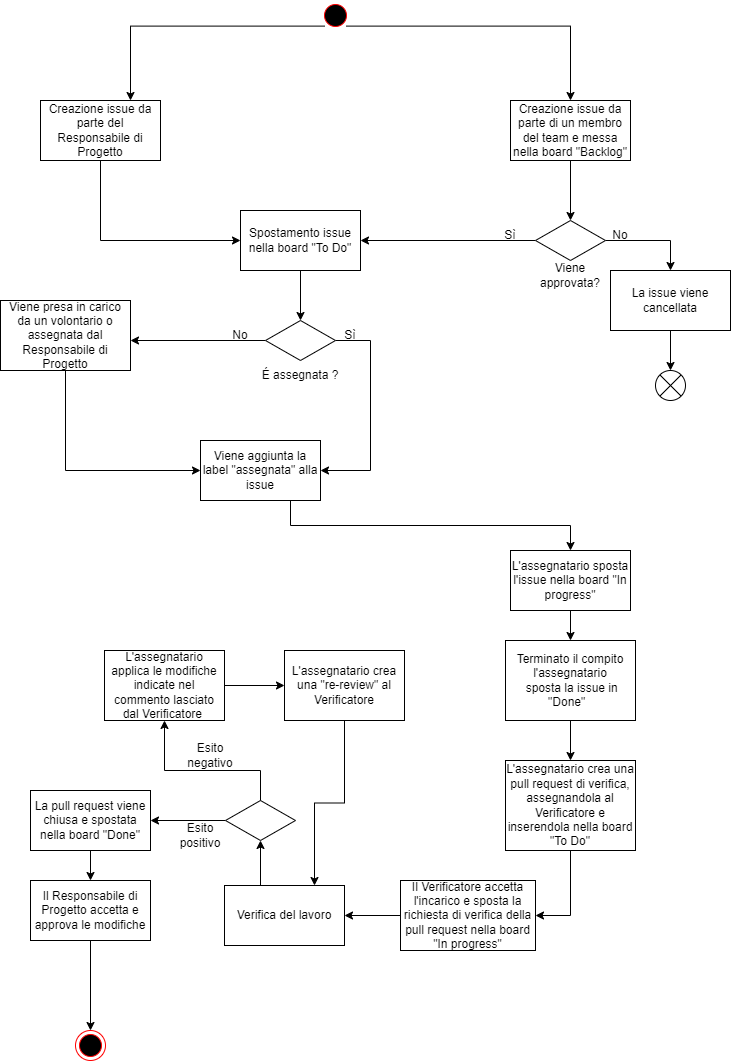
\includegraphics[scale=0.5]{Contenuto/Immagini/ticket.png}
\caption{Attività di gestione dei ticket}
\end{figure}

Note:
\begin{itemize}
\item Viene data a tutti i membri la possibilità di proporre un ticket per snellire la procedura;
\item Il Responsabile di Progetto può decidere di scomporre un ticket in "sotto-ticket" quando ritiene che questo sia troppo complesso;
\item In generale i membri sono tenuti a dare titoli e descrizioni concise e coerenti dei ticket che creano, non saranno accettati ticket con corpo vuoto o ticket senza scadenza.
\end{itemize}

\paragraph{Metriche}
Le metriche adottate per la valutazione del processo di pianificazione sono le seguenti:
\begin{itemize}
\item \textbf{MPC02 Budgeted cost of work scheduled};
\item \textbf{MPC03 Actual cost of work performed};
\item \textbf{MPC05 Schedule variance};
\item \textbf{MPC06 Budget variance}.
\end{itemize} 
Per maggiori informazioni consultare §B.

\paragraph{Strumenti}
Per il supporto all’attività di pianificazione di progetto è stato scelto come strumento
\textbf{GanttProject}, software open-source e multi-piattaforma usato per la realizzazione di diagrammi di Gantt. Servirà per tenere traccia dell'assegnazione delle risorse, del rispetto delle scadenze e dell'analisi dei carichi di lavoro.


\subsection{Formazione dei membri del team}
Il processo di formazione ha lo scopo di assicurare che ogni membro abbia le conoscenze necessarie per svolgere i compiti che gli vengono assegnati e deve garantire il mantenimento di un personale competente nel tempo.

\subsubsection{Obiettivi}
Il processo mira al mantenimento costante (auspicabilmente per tutta la durata del progetto) di membri competenti ed esperti e garantisce quindi qualità di lavoro in linea con le aspettative.

\subsubsection{Formazione interna}
Ogni membro dovrà provvedere alla propria formazione in maniera autonoma, approfondendo le proprie mancanze con lo studio personale. I membri più esperti potranno condividere le loro conoscenze e/o materiale con il resto del team. In ogni momento un membro che trova difficoltà nell'esecuzione di un compito può rivolgersi al Responsabile di Progetto che dovrà organizzare le attività necessarie per l'apprendimento. Si farà riferimento alla documentazione seguente, ma essendo non esaustiva è consigliato un approfondimento con materiale reperito di proprio conto:
\begin{itemize}
\item \textbf{\LaTeX}: \mylink{https://www.latex-project.org/help/documentation/};
\item \textbf{GitHub}: \mylink{https://docs.github.com/};
\item \textbf{Git}: \mylink{https://git-scm.com/doc};
\item \textbf{AWS Cognito}\textsuperscript{G}: \mylink{https://docs.aws.amazon.com/cognito/latest/developerguide/};
\item \textbf{AWS Comprehend}\textsuperscript{G}: \mylink{https://docs.aws.amazon.com/comprehend/};
\item \textbf{API Gateway}\textsuperscript{G}: \mylink{https://docs.aws.amazon.com/apigateway/latest/developerguide/};
\item \textbf{AWS Lambda}\textsuperscript{G}: \mylink{https://docs.aws.amazon.com/lambda/};
\item \textbf{AWS Amplify}\textsuperscript{G}: \mylink{https://aws.amazon.com/it/amplify/};
\item \textbf{AWS Rekognition}\textsuperscript{G}: \mylink{https://aws.amazon.com/it/rekognition/}.
\end{itemize}

\subsubsection{Formazione esterna}
L'azienda proponente \zd ha deciso di offrire ai membri del team una formazione specifica sulle tecnologie da loro richieste. L'azienda fornirà di volta in volta risorse informative sul canale Slack apposito, con lo scopo di fornire già una minima preparazione prima degli incontri formativi. Ogni membro è tenuto ad uno studio personale del materiale condiviso prima di ogni incontro.


\subsubsection{Strumenti a supporto della gestione organizzativa}
Il team userà i seguenti strumenti per supportare il processo di gestione organizzativa:
\begin{itemize}
\item \textbf{Slack}: strumento standard usato dal team per la comunicazione interna e con il proponente;
\item \textbf{Telegram}: strumento di messaggistica usato dal team per decisione e questioni meno importanti; 
\item \textbf{Git}: strumento utilizzato per il versionamento;
\item \textbf{GitHub}: strumento utilizzato per il versionamento e per il salvataggio di tutti i file prodotti dai membri del team; 
\item \textbf{GitHub Issues}: sistema integrato in GitHub usato per la gestione dei ticket;
\item \textbf{Google Drive}: utilizzato per la condivisione di documenti che richiedono molti cambiamenti dove la modifica in tempo reale è richiesta;
\item \textbf{Gmail}: servizio di posta elettronica scelto dal gruppo;
\item \textbf{Zoom}: strumento usato all'inizio per fare riunioni tra membri del team;
\item \textbf{Discord}: strumento standard usato per le riunioni tra i membri del team. 
\end{itemize}

	
	
\end{document}